\documentclass[11pt]{article}
\usepackage[margin=1in]{geometry}
\usepackage{amsmath,amssymb,amsthm,mathtools}
\usepackage{tikz,tikz-cd}
\usepackage{amsmath,amssymb}
\usetikzlibrary{arrows.meta,decorations.markings,backgrounds,cd,calc}
\colorlet{c1}{blue!70!black}\colorlet{c2}{red!70!black}\colorlet{c3}{green!45!black}
\tikzset{
 ->-/.style={decoration={markings,mark=at position .55 with {\arrow{Stealth[length=2.4mm]}}},postaction={decorate}},
 ->>-/.style={decoration={markings,mark=at position .5 with {\arrow{Stealth[length=2.4mm]}},mark=at position .6 with {\arrow{Stealth[length=2.4mm]}}},postaction={decorate}},
 every picture/.append style={show background rectangle, background rectangle/.style={fill=white}}
}

\usepackage{enumitem}
\usepackage[most]{tcolorbox}
\usepackage[colorlinks=true,linkcolor=blue!60!black]{hyperref}

\newcommand{\Z}{\mathbb Z}
\newcommand{\RP}{\mathbb{RP}}
\newcommand{\Hred}{\tilde H}
\newcommand{\im}{\operatorname{im}}
\newtcolorbox{note}{colback=gray!6,colframe=gray!60,boxrule=0.5pt,arc=2pt}
\setlength{\parindent}{0pt}\setlength{\parskip}{4pt}
\emergencystretch=3em

\title{MATH730 Midterm II practice --- solutions}
\date{}
\begin{document}
\maketitle
\vspace{-2.5em}

%=====================================================
\section*{Problem 1: a $\Delta$-complex structure on $\RP^2$ and its homology}

\textbf{The $\Delta$-complex.} $\RP^2$ is the square $[0,1]^2$ with opposite boundary points identified antipodally: $(x,0)\sim(1-x,1)$ and $(0,y)\sim(1,1-y)$. Label the corners $P_0=(0,0)$, $P_1=(1,0)$, $P_2=(1,1)$, $P_3=(0,1)$. The identifications glue $P_0\sim P_2$ and $P_1\sim P_3$, giving two vertices $v$ and $w$. Cut the square along the diagonal from $P_1$ to $P_3$:
\begin{center}
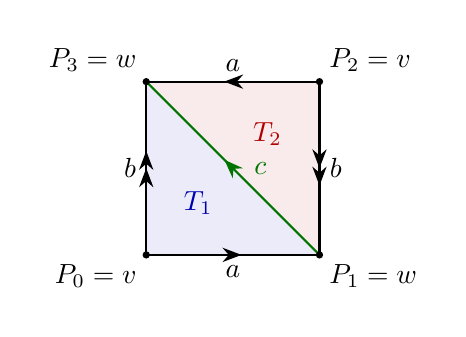
\begin{tikzpicture}[scale=2.2]
\coordinate (P0) at (0,0); \coordinate (P1) at (1,0); \coordinate (P2) at (1,1); \coordinate (P3) at (0,1);
\fill[c1!8] (P0)--(P1)--(P3)--cycle; \fill[c2!8] (P1)--(P2)--(P3)--cycle;
\draw[thick,->-] (P0)--node[below]{$a$}(P1);
\draw[thick,->-] (P2)--node[above]{$a$}(P3);
\draw[thick,->>-] (P0)--node[left]{$b$}(P3);
\draw[thick,->>-] (P2)--node[right]{$b$}(P1);
\draw[thick,c3,->-] (P1)--node[pos=0.42,above right=-1pt]{$c$}(P3);
\node[below left] at (P0){$P_0=v$}; \node[below right] at (P1){$P_1=w$};
\node[above right] at (P2){$P_2=v$}; \node[above left] at (P3){$P_3=w$};
\node[c1] at (0.3,0.3){$T_1$}; \node[c2] at (0.7,0.7){$T_2$};
\foreach \p in {P0,P1,P2,P3} \fill (\p) circle(0.6pt);
\end{tikzpicture}
\end{center}
\begin{itemize}
\item Vertices: $v=P_0=P_2$ and $w=P_1=P_3$.
\item Edges: $a=[P_0,P_1]=[P_2,P_3]$ (bottom and top, glued), $b=[P_0,P_3]=[P_2,P_1]$ (left and right, glued), and $c=[P_1,P_3]$ (the diagonal).
\item 2-simplices: $T_1=[P_0,P_1,P_3]$ and $T_2=[P_2,P_1,P_3]$.
\end{itemize}
This is a valid $\Delta$-complex. In each triangle the vertex order is compatible with all three edge arrows: in $T_1$ the order is $P_0<P_1<P_3$, and in $T_2$ it is $P_2<P_1<P_3$. The two edges being glued (bottom and top, left and right) are identified by the linear map that respects these orders. The open simplices are disjoint and cover $\RP^2$.

\textbf{Boundary maps.} Using $\partial[u_0,u_1,u_2]=[u_1,u_2]-[u_0,u_2]+[u_0,u_1]$:
\begin{align*}
\partial T_1&=[P_1,P_3]-[P_0,P_3]+[P_0,P_1]=c-b+a,\\
\partial T_2&=[P_1,P_3]-[P_2,P_3]+[P_2,P_1]=c-a+b,\\
\partial a&=w-v,\qquad \partial b=w-v,\qquad \partial c=w-w=0.
\end{align*}
The chain complex is $0\to\Z^2\xrightarrow{\partial_2}\Z^3\xrightarrow{\partial_1}\Z^2\to0$, with bases $\{T_1,T_2\}$, $\{a,b,c\}$, $\{v,w\}$.

\textbf{$H_0$.} $\im\partial_1=\langle w-v\rangle$, so $H_0=\Z\langle v,w\rangle/\langle w-v\rangle\cong\Z$.

\textbf{$H_1$.} $\partial_1(xa+yb+zc)=(x+y)(w-v)$, so $\ker\partial_1=\{y=-x\}$, which is free with basis $\{a-b,\ c\}$. In this basis
\[\partial T_1=(a-b)+c\ \leftrightarrow\ (1,1),\qquad \partial T_2=-(a-b)+c\ \leftrightarrow\ (-1,1).\]
Change the basis of the image: $\langle(1,1),(-1,1)\rangle=\langle(1,1),(0,2)\rangle$, and $f_1=(1,1)$, $f_2=(0,1)$ form a basis of $\Z^2$. Hence
\[H_1=\ker\partial_1/\im\partial_2\cong\Z\langle f_1,f_2\rangle/\langle f_1,\,2f_2\rangle\cong\Z/2,\]
generated by $[c]$. (Check: the matrix with rows $(1,1)$ and $(-1,1)$ has determinant $2$, so the quotient has order $2$.)

\textbf{$H_2$.} $\partial_2(pT_1+qT_2)=(p-q)(a-b)+(p+q)c$. This is $0$ only if $p=q$ and $p=-q$, i.e.\ $p=q=0$. So $\ker\partial_2=0$ and $H_2=0$.

\[\boxed{H_0(\RP^2)=\Z,\quad H_1(\RP^2)=\Z/2,\quad H_2(\RP^2)=0,\quad H_k(\RP^2)=0\ (k\ge3).}\]

\begin{note}
Why $H_2=0$: the two triangles can't be signed so that the $c$ terms cancel while the $a$ and $b$ terms also cancel. This is the algebraic shadow of $\RP^2$ being non-orientable. For the torus, the same computation gives $\partial T_1=\partial T_2$, so $T_1-T_2$ is a cycle.
\end{note}

%=====================================================
\section*{Problem 2}

\textbf{(a)} Let $f,g:C_\bullet\to D_\bullet$ be chain maps. They are \textbf{chain homotopic} if there are homomorphisms $P_n:C_n\to D_{n+1}$, for all $n$, such that
\[\partial^D_{n+1}\circ P_n+P_{n-1}\circ\partial^C_n=g_n-f_n\qquad\text{for all }n.\]
$P$ is called a chain homotopy. (Consequence worth stating: then $f_*=g_*$ on homology, since for a cycle $z$ we get $g(z)-f(z)=\partial P(z)$, a boundary.)

\textbf{(b)} Write the short exact sequence as $0\to A_\bullet\xrightarrow{i}B_\bullet\xrightarrow{j}C_\bullet\to0$. Let $[z]\in H_k(C)$, so $z\in C_k$ with $\partial z=0$.
\begin{enumerate}
\item \textbf{Lift.} Since $j$ is surjective, choose $b\in B_k$ with $j(b)=z$.
\item \textbf{Take the boundary.} Consider $\partial b\in B_{k-1}$. Since $j$ is a chain map, $j(\partial b)=\partial j(b)=\partial z=0$. So $\partial b\in\ker j=\im i$.
\item \textbf{Pull back.} Since $i$ is injective, there is a unique $a\in A_{k-1}$ with $i(a)=\partial b$.
\item \textbf{$a$ is a cycle.} $i(\partial a)=\partial i(a)=\partial\partial b=0$, and $i$ is injective, so $\partial a=0$.
\item \textbf{Define} $d([z])=[a]\in H_{k-1}(A)$.
\end{enumerate}
\textbf{Well defined:}
\begin{itemize}
\item Another lift of $z$ has the form $b'=b+i(a')$ with $a'\in A_k$ (because $j(b'-b)=0$). Then $\partial b'=\partial b+i(\partial a')$, so $a$ becomes $a+\partial a'$, which is in the same homology class.
\item Another representative of the class is $z'=z+\partial c$ with $c\in C_{k+1}$. Lift $c$ to $\tilde c\in B_{k+1}$. Then $b+\partial\tilde c$ lifts $z'$, and $\partial(b+\partial\tilde c)=\partial b$, so we get the same $a$.
\end{itemize}
Summary: \emph{lift $z$ to $B$, take the boundary, pull back to $A$.}
\[\begin{tikzcd}[row sep=small]
 & b \arrow[r,mapsto,"j"]\arrow[d,mapsto,"\partial"'] & z\\
 a\arrow[r,mapsto,"i"] & \partial b &
\end{tikzcd}\]

%=====================================================
\section*{Problem 3: attaching an $(n+2)$-cell}

\textbf{Setup.} Let $\varphi:S^{n+1}\to X$ be the attaching map, $Y=X\cup_\varphi D^{n+2}$, $q:X\sqcup D^{n+2}\to Y$ the quotient map, $e=q(\operatorname{int}D^{n+2})$ the open cell, and $0=q(0)$ its center. Set
\[A=Y\setminus\{0\},\qquad B=e.\]
\begin{itemize}
\item $A$ and $B$ are open in $Y$, and $A\cup B=Y$.
\item $B\cong\operatorname{int}D^{n+2}$ is contractible, so $\Hred_*(B)=0$.
\item $A$ deformation retracts onto $X$ via $H_t(x)=(1-t)x+t\,x/|x|$ on $D^{n+2}\setminus\{0\}$ and the identity on $X$. This is well defined on the quotient because it fixes $S^{n+1}$ pointwise. So $\Hred_*(A)\cong\Hred_*(X)$.
\item $A\cap B\cong\operatorname{int}D^{n+2}\setminus\{0\}$ deformation retracts onto a sphere $\{|x|=\tfrac12\}$, so $A\cap B\simeq S^{n+1}$. In particular $A\cap B\neq\emptyset$, and $\Hred_k(A\cap B)\cong\Z$ for $k=n+1$ and $0$ otherwise.
\end{itemize}
Since $A\cap B\neq\emptyset$, reduced Mayer--Vietoris gives exact sequences
\[\Hred_k(A\cap B)\to\Hred_k(A)\oplus\Hred_k(B)\to\Hred_k(Y)\to\Hred_{k-1}(A\cap B)\to\Hred_{k-1}(A)\oplus\Hred_{k-1}(B).\]
Substituting the above, with $\Hred_k(X)=H_k(X)=0$ for $k>n$:
\[\Hred_k(S^{n+1})\to\Hred_k(X)\to\Hred_k(Y)\to\Hred_{k-1}(S^{n+1})\to\Hred_{k-1}(X).\tag{$*$}\]

\textbf{Case $k\le n$.} Here $k\neq n+1$ and $k-1\neq n+1$, so both sphere terms in $(*)$ vanish:
\[0\to\Hred_k(X)\to\Hred_k(Y)\to0.\]
So $\Hred_k(Y)\cong\Hred_k(X)$, induced by the inclusion. For $k\ge1$ this says $H_k(Y)\cong H_k(X)$. For $k=0$, $H_0\cong\Hred_0\oplus\Z$ for nonempty spaces, so $H_0(Y)\cong H_0(X)$ as well. (Both are $\Z$: $X$ is connected, and so is $Y$, being $X$ union the connected set $q(D^{n+2})$, which meets $X$.)

\textbf{Case $k=n+1$.} $(*)$ reads
\[\Hred_{n+1}(X)=0\to\Hred_{n+1}(Y)\to\Hred_n(S^{n+1})=0,\]
so $H_{n+1}(Y)=0$.

\textbf{Case $k=n+2$.} $(*)$ reads
\[\Hred_{n+2}(X)=0\to\Hred_{n+2}(Y)\xrightarrow{d}\Hred_{n+1}(S^{n+1})=\Z\to\Hred_{n+1}(X)=0,\]
so $d$ is an isomorphism and $H_{n+2}(Y)\cong\Z$.

\textbf{Case $k>n+2$.} Then $k>n$ and $k-1>n+1$, so $(*)$ reads $0\to\Hred_k(Y)\to0$ and $H_k(Y)=0$.

\begin{note}
Why the attaching map didn't matter: the only nonzero sphere term is $\Hred_{n+1}(S^{n+1})$, and the map out of it, $\varphi_*$, lands in $\Hred_{n+1}(X)=0$. Compare the torus or Klein bottle, where the cell is attached one dimension above the top homology of $X$. There $\varphi_*:\Z\to H_1(X)$ is a genuine map and decides the answer. The ``$+2$'' in the problem is exactly what makes $\varphi_*$ automatically zero.
\end{note}

\end{document}
